159. \begin{figure}[ht!]
\center{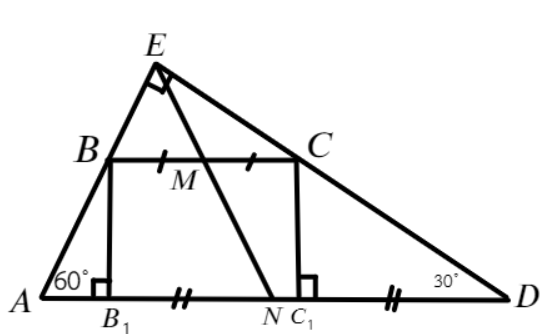
\includegraphics[scale=0.35]{g8-159.png}}
\end{figure}\\
а) Опустим высоты $BB_1$ и $CC_1,$ тогда $BCC_1B_1$ является прямоугольником и $B_1C_1=BC=4$см. Пусть $AB_1=x,$ тогда $DC_1=6-x.$ Выразим высоты из треугольников
$ABB_1$ и $DCC_1:\ BB_1=AB_1\ tg(60^\circ)=\sqrt{3}x=CC_1\ tg(30^\circ)=\cfrac{\sqrt{3}}{3}(6-x),$ откуда $\sqrt{3}x=\cfrac{\sqrt{3}}{3}(6-x),\ 3x=6-x,\ x=\cfrac{3}{2}$см. Тогда $BB_1=CC_1=\cfrac{3\sqrt{3}}{2}$см и по теореме Пифагора $AB=\sqrt{\cfrac{9}{4}+\cfrac{27}{4}}=3$см,$ CD=\sqrt{\cfrac{81}{4}+\cfrac{27}{4}}=
3\sqrt{3}$см.\\
б) Площадь равна $S=\cfrac{3\sqrt{3}}{2}\cdot\cfrac{4+10}{2}=\cfrac{21\sqrt{3}}{2}\text{ см}^2.$\\
в) Продлим боковые стороны трапеции до пересечения, тогда точка их пересечения лежит на одной прямой с серединами оснований (и с точкой пересечения диагоналей, но в нашей задаче это не требуется). Тогда $\angle AED=180^\circ-30^\circ-60^\circ=90^\circ.$ Отрезки $EN$ и $EM$ являются медианами, проведёнными из прямого угла, значит $MN=EN-EM=\cfrac{1}{2}AD-\cfrac{1}{2}BC=\cfrac{1}{2}(AD-BC)=\cfrac{1}{2}\cdot6=3$см.\\
